\section{Funzioni} \label{sec_funzioni}

\dfn{
	Dati due insiemi $A \neq \emptyset$ e $B \neq \emptyset$, una \textbf{funzione} $f$ da $A$ a $B$ 
	\begin{equation*}
		f: A \to B
	\end{equation*}
	è una corrispondenza univoca da $A$ a $B$. Ovvero associa ad ogni $x \in A$ uno e un solo $y \in B$. Tale elemento è il \textbf{valore della funzione} in $x$ e si scrive. 
	\begin{equation*}
		f(x) = y
	\end{equation*}
	Questa associazione di un elemento di $A$ ad un elemento di $B$ è data dalla \textbf{legge di associazione}: 
	\begin{equation*}
		\forall x\in A, \exists\oc y\in B : f(x) = y
	\end{equation*}

	    
	L'insieme $A$ è il \textbf{dominio} della funzione, mentre l'insieme $B$ è il \textbf{codominio} della funzione.  L'insieme dei valori di una funzione è invece l'\textbf{immagine} (si ottiene proiettando la funzione sull'asse y):
	\begin{equation*}
		\mathrm{Im}f = \left\{y \in B\,\middle|\, \exists x \in A : f(x) = y\right\}
	\end{equation*}
}

Una funzione può essere anche chiamata \textit{corrispondenza} oppure \textit{mappa}. Essa è definita quindi da tre cose:
\begin{enumerate}
    \item Un \textbf{dominio}
    \item Un \textbf{codominio}
    \item Una \textbf{legge di associazione}
\end{enumerate}


Affinché due funzioni siano uguali, il dominio, il codominio e la legge di associazione devono corrispondere. In altri termini date due funzioni $f: A \to B$ e $g: A' \to B'$, le funzioni risultano uguali se e solo se:

\begin{equation*}
    \begin{cases}
    A = A'\\
    B = B'\\
    f = g
    \end{cases}
\end{equation*}

Esempio: data $f: \mathbb{R} \to \mathbb{R}\;\, f(x) = x^2$ e $g: \mathbb{R} \to \mathbb{R}_{+}\;\, g(x) = x^2$, le due funzioni sono diverse in quanto la seconda ha un codominio diverso dalla prima ($\mathbb{R}_{+} = \{x \in \mathbb{R}\, |\, 0 \leq x\}$).\\

\imp{
Il \textbf{dominio naturale} di una funzione è il più grande sottoinsieme in cui quella funzione è definita.
}

\subsection{Funzione iniettiva (1-1)}

\dfn{
    Una funzione $f: A \to B$ è detta iniettiva se e solo se:
    \begin{equation*}
        \forall x, y \in A : x \neq y \implies f(x) \neq f(y)
    \end{equation*}
    o equivalentemente:
    \begin{equation*}
        \forall x, y \in A :  f(x) = f(y) \implies x = y
    \end{equation*}
}

Spesso l'iniettività di una funzione viene più brevemente indicata con (1-1). Inoltre questa proprietà dipende strettamente da come viene "scelto il dominio":

\begin{table}[H]
\centering
\begin{tabular}{ll}
$f: \mathbb{R} \to \mathbb{R}\;\, f(x) = x^3$          & È iniettiva      \\
$f: \mathbb{R} \to \mathbb{R}\;\, f(x) = x^2$        & Non è iniettiva  \\
$f: \mathbb{R}_{+} \to \mathbb{R}\;\, f(x) = x^2$ & È iniettiva     
\end{tabular}
\end{table}

La seconda funzione infatti non è iniettiva ($f(-2) = f(2) = 4$), mentre la terza lo è in quanto il dominio è stato ristretto.

\subsection{Funzione suriettiva (Su)}

\dfn{
    Una funzione $f: A \to B$ è detta suriettiva se e solo se:
    \begin{equation*}
        \forall b \in B, \exists a \in A : f(a) = b
    \end{equation*}
}

Spesso la suriettività di una funzione viene più brevemente indicata con (Su). Inoltre questa proprietà dipende strettamente da come viene "scelto il codominio":

\begin{table}[H]
\centering
\begin{tabular}{ll}
$f: \mathbb{R} \to \mathbb{R}\;\, f(x) = x^3$          & È suriettiva      \\
$f: \mathbb{R} \to \mathbb{R}\;\, f(x) = x^2$        & Non è suriettiva  \\
$f: \mathbb{R} \to \mathbb{R}_{+}\;\, f(x) = x^2$ & È suriettiva     
\end{tabular}
\end{table}

La seconda funzione infatti non è iniettiva ($f(x) = -2$ non ha soluzione per esempio), mentre la terza lo è in quanto il codominio è stato ristretto.

\subsection{Funzione biunivoca}

\dfn{
	Una funzione viene detta \textbf{biunivoca} (o biettiva) se è \textbf{iniettiva (1-1)} e \textbf{suriettiva (Su)}.
}
Le funzioni biunivoche sono molto importanti perché ci permettono di definire le funzioni inverse. In pratica se una funzione ha questa proprietà significa che ad un elemento del codominio è associato uno e un solo elemento del dominio, ed inoltre tutti gli elementi del codominio hanno un corrispettivo nel dominio: in pratica l'immagine coincide con il codominio.

\subsection{Funzione invertibile}
Le funzioni inverse sono tutte quelle funzioni che ci permettono di passare da un elemento nell'immagine di un'altra funzione al valore associato ad esso nel dominio. Alcuni esempi di funzioni e il loro inverso (che vedremo più avanti) sono il \textit{seno} e \textit{arcoseno}, \textit{esponenziale} e \textit{logaritmo}, \textit{potenze} e \textit{radici}, ecc. Non tutte le funzioni sono invertibili, anzi molto poche perché una funzione, affinché risulti invertibile, è necessario che sia \textbf{biunivoca}.

\dfn{
    Una funzione $f: A\to B $ si dice \textbf{invertibile} se $\exists \, f^{-1}: B\to A$ tale che:
    \begin{align*}
        \forall a \in A: f^{-1}(f(a)) = a\\
        \forall b \in B: f(f^{-1}(b))= b
    \end{align*}
}

\subsection{Funzioni crescenti e decrescenti}
\dfn{
    Data una funzione $f: I \to \mathbb{R}$ dove $I \subseteq \mathbb{R}$:
    \begin{enumerate}
        \item $f$ si dice \textbf{crescente} (o \textbf{monotona}) se:
            \begin{equation*}
                \forall x,y \in I : x < y \implies f(x) \leq f(y)
            \end{equation*}
            Se al posto del \textit{minore o uguale} ($\leq$) avessimo usato un \textit{minore stretto} ($<$) la proprietà era più forte, e in quel caso la funzione sarebbe stata \textbf{strettamente crescete}.
        \item $f$ si dice \textbf{decrescente} (o \textbf{monotona decrescente}) se:
            \begin{equation*}
                \forall x,y \in I : x < y \implies f(x) \geq f(y)
            \end{equation*}
            Se al posto del \textit{maggiore o uguale} ($\geq$) avessimo usato un \textit{maggiore stretto} ($>$) la funzione sarebbe stata \textbf{strettamente decrescete}.
    \end{enumerate}
}

\subsection{Funzioni pari e dispari}
Un modo per classificare una funzione è vedere se è pari, dispari, o nessuna delle due. Ne consegue che non per forza una funzione deve essere pari o dispari. E inoltre se una funzione non è pari non è detto che sia dispari.
\dfn{
    Data una funzione $f: A \to \mathbb{R}$, se:
    \begin{equation}
        f(-x) = f(x) \qquad \forall x \in A\\
    \end{equation}
    La funzione si dice \textbf{pari}. Mentre se:
    \begin{equation}
        f(-x) = -f(x) \qquad \forall x \in A\\
    \end{equation}
    La funzione si dice \textbf{dispari}.
}
La nomenclatura pari o dispari deriva dalle potenze, in quanto $(-a)^n = a^n$ se $n$ è pari, mentre $(-a)^n = -a^n$ se $n$ è dispari.\\

Le funzioni pari hanno il grafico simmetrico rispetto all'asse delle ordinate, mentre le funzioni dispari sono simmetriche rispetto all'origine.

\subsection{Valore assoluto}

\dfn{
    Dato un numero $a \in \mathbb{R}$ si dice \textbf{valore assoluto di $a$}:
    \begin{equation*}
        |a| \vcentcolon = \mathrm{max}(a, -a)
    \end{equation*}
}

Il valore assoluto si espande nel seguente modo:
\begin{itemize}
    \item $|a| \leq b \quad \mathrm{con}\;\, b > 0 \iff -b \leq a \leq b$
    \item $|a| \geq b \quad \mathrm{con}\;\, b > 0 \iff a \leq -b \lor a \geq b$
\end{itemize}

\subsection{Fattoriale}
\dfn{
Dato un numero $n \in \mathbb{N}$, il \textbf{fattoriale} di $n$ è definito:
\begin{equation*}
    n!=
    \begin{cases}
    1 \qquad \qquad \qquad \qquad \qquad \qquad \,\mathrm{se}\;\, n = 0\\
    1\cdot 2 \cdot 3 \cdot 4 \cdot \dots (n-1) \cdot n \qquad \mathrm{se}\;\, n \geq 1
    \end{cases}
\end{equation*}
oppure in maniera ricorsiva:
\begin{equation*}
    n! =
    \begin{cases}
    1 \qquad \qquad \qquad \, \mathrm{se}\;\, n = 0\\
    n \cdot (n-1)! \qquad \mathrm{se}\;\, n \geq 1
    \end{cases}
\end{equation*}
}
Il fattoriale è solo una notazione introdotta per evitare di scrivere moltiplicazioni ripetute di numeri naturali.

\subsection{Coefficiente binomiale} \label{sec_coefficiente-binomiale}

\dfn{
Dati due numeri $n, m \in \mathbb{N}: m \leq n$ si definisce \textbf{coefficiente binomiale}:
\begin{equation*}
\binom{n}{m}=
    \begin{cases}
    1 \qquad \qquad \qquad \, \mathrm{se}\;\, m = 0\\
    \dfrac{n!}{(n-m)!m!} \quad \;\, \mathrm{se}\;\, m \geq 1\\
    \end{cases}
\end{equation*}
}

Un modo per ricordarselo è pensare che il coefficiente binomiale di $n$ su $m$ rappresenta il numero di sottoinsiemi di $m$ elementi in un insieme di $n$ elementi.\\
Gode delle seguenti proprietà:
\begin{align*}
    1) &\qquad\binom{n}{k} = \binom{n}{n-k}\\[0.2cm]
    2) &\qquad\binom{n}{k-1} + \binom{n}{k} = \binom{n+1}{k}
\end{align*}

\subsubsection{Coefficiente binomiale generalizzato} \label{sec_coefficiente-binomiale-gen}
Dato il coefficiente binomiale appena definito:
\begin{equation*}
\binom{n}{m}=
    \begin{cases}
    1 \qquad \qquad \qquad \, \mathrm{se}\;\, m = 0\\
    \dfrac{n!}{(n-m)!m!} \quad \;\, \mathrm{se}\;\, m \geq 1\\
    \end{cases}
\end{equation*}
Il caso $m \geq 1$ è possibile riscriverlo come segue:
\begin{equation*}
	\binom{n}{m} = \dfrac{n!}{(n-m)!m!} = \dfrac{m (m - 1) (m -2) \cdots (m - n + 1)}{n!}
\end{equation*}
Questo permette di togliere l'operazione fattoriale dal primo argomento e quindi permette di generalizzare la sua definizione a $n \in \mathbb{R}$. In questo caso si parla di coefficiente binomiale generalizzato (con $\alpha \in \mathbb{R}$):
\begin{equation*}
	\binom{\alpha}{m} = 
		\begin{cases}
			1 \qquad \qquad \qquad \qquad \qquad \qquad \qquad \,\; \mathrm{se}\;\, \alpha = 0\\[5pt]
		\dfrac{\alpha (\alpha - 1) (\alpha -2) \cdots (\alpha - n + 1)}{n!} \quad \;\, \mathrm{se}\;\, \alpha \geq 1\\
		\end{cases}
\end{equation*}



\subsection{Binomio di Newton} \label{sec_binomioNewton}
Il binomio di Newton è metodo per esprimere lo sviluppo della potenza \textit{n}-esima di un binomio qualsiasi mediante una formula.
\subsubsection{Sommatoria} \label{sec_sommatoria}
Prima però di introdurlo è necessario introdurre una notazione spesso usata in matematica per scrivere in maniera più agevole somme di un certo numero di addendi:
\dfn{
La \textbf{sommatoria} si indica con la lettera sigma maiuscola $(\Sigma)$, prevede un indice (generalmente $i$, $j$ o $k$), un'espressione algebrica a destra della lettera sigma in cui viene usato l'indice e due valori per l'indice: uno di partenza e l'altro di terminazione, rispettivamente indicati sotto e sopra sigma. La notazione generale diventa quindi:
\begin{equation*}
    \sum_{k=m}^{n} f(k) = f(m) + f(m + 1) + f(m + 2) + \dots + f(n-1) + f(n)
\end{equation*}
Da notare che la sommatoria espande il termine $f(k)$ sostituendo a $k$ ogni singolo numero naturale compreso tra $m$ ed $n$ per poi sommare tutti i termini insieme. \textbf{È necessario quindi che} $\mathbf{m\leq n}$.
}

\subsubsection{Binomio di Newton (effettivo)}
L'idea alla base del binomio di Newton è cercare di trovare una formula che semplifichi lo sviluppo in potenza di un binomio qualsiasi. Esiste quindi un modo per sviluppare $(a+b)^n$ senza dover per forza fare tutte le moltiplicazioni intermedie? Proviamo ad elencare gli sviluppi del binomio per i primi valori di $n$:
\begin{align*}
    (a+b)^2 &= a^2 + 2ab + b^2\\
    (a+b)^3 &= a^3 + 3a^2b + 3ab^2 + b^3\\
    (a+b)^4 &= a^4 + 4a^3b + 6a^2b^2 + 4ab^3 + b^4\\
    \vdots \qquad
\end{align*}
Tralasciando momentaneamente i coefficienti è facile notare un certo schema nelle potenze di $a$ e di $b$:
\begin{equation*}
    (a+b)^n = a^nb^0 + a^{n-1}b^1 + \dots + a^1b^{n-1} + a^0b^n
\end{equation*}
Per i coefficienti non faremo la dimostrazione ma sono legati al coefficiente binomiale (Sezione \ref{sec_coefficiente-binomiale}), infatti:
\begin{align*}
    (a+b)^2 &= \binom{2}{2}a^2 + \binom{2}{1}ab + \binom{2}{0}b^2 = \\[2pt]
    &= \dfrac{2!}{(2-2)!2!}a^2 + \dfrac{2!}{(2-1)!1!}ab + \dfrac{2!}{(2-0)!0!}b^2 =\\[5pt]
    &= 1\cdot a^2 + 2\cdot ab + 1 \cdot b^2
\end{align*}

Di conseguenza il caso generale diventa:
\begin{equation*}
    (a+b)^n = \binom{n}{n} a^n b^0 + \binom{n}{n-1} a^{n-1} b^1 + \dots + \binom{n}{1} a^1b^{n-1} + \binom{n}{0} a^0b^n = 
\end{equation*}
Introducendo la notazione di sommatoria (\ref{sec_sommatoria}) per semplificare e utilizzando qualche proprietà del coefficiente binomiale (\ref{sec_coefficiente-binomiale}):
\begin{equation*}
    = \sum \limits_{k = 0}^{n} \binom{n}{n-k} a^{n-k}b^k = \sum \limits_{k = 0}^{n} \binom{n}{k} a^{n-k}b^k
\end{equation*}

\dfn{
Il \textbf{binomio di Newton} esprime lo sviluppo della potenza \textit{n}-esima di un binomio qualsiasi mediante la formula:
\begin{equation*}
    (a+b)^n = \sum \limits_{k=0}^{n} \binom{n}{k} a^{n-k} b^k
\end{equation*}
}


\subsection{Radice aritmetica} \label{sec_radiceAritmetica}
\thm{
La radice di un numero reale positivo esiste sempre ed è unica:
\begin{equation*}
    \forall a\in \mathbb{R}_{+}, \;\forall n\in \mathbb{N}\setminus\{0\}, \exists \oc b\in \mathbb{R}_{+}: b^n = a
\end{equation*}
$b$ si chiama radice \textbf{aritmetica \textit{n}-esima} di $a$ e si scrive $\sqrt[n]{a} \vcentcolon = b$. In quanto $b\in \mathbb{R}_{+}$ la radice aritmetica è \textbf{sempre positiva}.
}
Dimostriamo il teorema della radice n-esima semplificato, cioè solo per il caso in cui $n = 2$. Prima però è necessario dimostrare un lemma:

\mlem{
	$\forall x, y \in \mathbb{R}: x, y \geq 0$
	\begin{enumerate}[label=\Alph*)]
	    \item $x^2 \leq y^2 \iff x \leq y$
	    \item $x^2 \geq y^2 \iff x \geq y$
	    \item $x^2 = y^2 \iff x = y$
	    \item $x^2 < y \implies \exists \epsilon > 0: (x+\epsilon)^2 < y$
	    \item $x^2 > y \implies \exists \epsilon > 0: (x-\epsilon)^2 > y$
	\end{enumerate}
}
    
\pf{
	Assumiamo come ipotesi generale che: $\forall x, y \in \mathbb{R}: x, y \geq 0$.

\begin{enumerate}[label=(\Alph*)]
	\item Vogliamo dimostrare che 
		\begin{equation*}
			 x^2 \leq y^2 \iff x \leq y
		\end{equation*}
		\begin{align*}
			&x^2 \leq y^2\\
			&x^2 - y^2 \leq 0\\
			&(x+y)(x-y) \leq 0
		\end{align*}
		Ovviamente essendo $x, y \geq 0 \implies x+y \geq 0$, quindi possiamo dividere da ambo i lati:
		\begin{gather*}
			x-y \leq 0\\
			x \leq y
		\end{gather*}

	\item La dimostrazione di questo punto è identica al precedente, di conseguenza non verrà riportata.

	\item Vogliamo dimostrare che 
		\begin{equation*}
			x^2 = y^2 \iff x = y
		\end{equation*}
		Dai due punti precedenti:
		\begin{equation*}
			x^2 = y^2 \iff
			\begin{cases}
				x^2 \leq y^2 \iff x \leq y\\
				x^2 \geq y^2 \iff x \geq y
			\end{cases}
			\iff x = y
		\end{equation*}


	\item Vogliamo dimostrare che:
		\begin{equation*}
			x^2 < y \implies \exists \epsilon > 0: (x + \epsilon)^2 < y
		\end{equation*}
		Assumiamo $x^2 < y$ per dimostrare:
		\begin{equation*}
			\exists \epsilon > 0: (x + \epsilon)^2 < y
		\end{equation*}
		Prendiamo $0 < \epsilon < 1$ in modo che $\epsilon^2 < \epsilon$:
		\begin{equation*}
			(x+\epsilon)^2 = x^2 + 2x\epsilon + \epsilon^2
		\end{equation*}
		Sostituendo ora $\epsilon^2$ con $\epsilon$ possiamo affermare che:
		\begin{gather*}
			x^2 + 2x\epsilon + \epsilon^2 \leq\\
			\leq x^2 + 2x\epsilon + \epsilon =\\
			= x^2 + \epsilon(2x + 1)
		\end{gather*}
		È possibile ora scegliere $y$ in modo da soddisfare $x^2 + \epsilon(2x + 1) < y$?
		\begin{gather*}
			x^2 + \epsilon(2x + 1) < y\\
			\epsilon(2x + 1) < y - x^2\\
			\epsilon < \dfrac{y-x^2}{2x+1}
		\end{gather*}
		Si ricorda che $(2x+1) > 0$ per ipotesi generale ($x \geq 0$). Anche $y-x^2 > 0$ per ipotesi, quindi è possibile scegliere $\epsilon$ in maniera tale da verificare:
		\begin{equation*}
			0 < \epsilon < \dfrac{y-x^2}{2x+1}
		\end{equation*}

	\item Vogliamo dimostrare che:
		\begin{equation*}
			x^2 > y \implies \exists \epsilon > 0: (x - \epsilon)^2 > y
		\end{equation*}
		Assumiamo $x^2 > y$ per dimostrare:
		\begin{equation*}
			\exists \epsilon > 0: (x - \epsilon)^2 > y
		\end{equation*}
		Espandiamo il quadrato:
		\begin{equation*}
			(x-\epsilon)^2 = x^2 -2x\epsilon + \epsilon^2
		\end{equation*}
		Essendo $\epsilon^2 > 0$ e dovendo dimostrare un maggiore possiamo anche toglierlo in quanto se $x^2 -2x\epsilon > y$ sicuramente $x^2 -2x\epsilon + \epsilon^2 > y$:
		\begin{align*}
			x^2 -2x\epsilon &> y\\
			x^2 - y &> 2x\epsilon\\
			2x\epsilon < &x^2 - y\\
			\epsilon < &\dfrac{x^2-y}{2x}
		\end{align*}
		Sempre per il lemma generale $x > 0$ e per ipotesi $x^2-y > 0$. È quindi possibile scegliere un $\epsilon$ affinché la tesi si verifichi:
		\begin{equation*}
			0 < \epsilon < \dfrac{x^2-y}{2x}
		\end{equation*}
\end{enumerate}
\hfill Qed.
}    


\pf{
	Torniamo ora alla nostra dimostrazione principale. Vogliamo dimostrare che (visto che ci siamo ridotti solo al caso $n = 2$):
	\begin{equation*}
		\forall a\in \mathbb{R}_{+}, \exists \oc b\in \mathbb{R}_{+}: b^2 = a
	\end{equation*}
	Utilizzando la proprietà di completezza di $\mathbb{R}$ (Sezione: \ref{sec_completezzaR}) definiamo un insieme $A$ tale che:
	\begin{equation*}
		A = \{c \in \mathbb{R} | c \geq 0 \land c^2 \leq a\}
	\end{equation*}
	Visto che $0 \in A \implies A \neq \emptyset$.
	\begin{equation*}
		\forall c\in A: c^2 \leq a \leq (a+1) \leq (a+1)^2
	\end{equation*}
	Da lemma \textbf{A} $\implies$ $c \leq a + 1$. $a + 1$ quindi è un \textit{maggiorante} di $A$ e conseguentemente $A$ è \textit{superiormente limitato}. Dalla proprietà di completezza:
	\begin{equation*}
		\exists\; \mathrm{sup}A = \vcentcolon b \in \mathbb{R}_{+} 
	\end{equation*}
	Ci riduciamo quindi a dimostrare che $b^2 = a$, cosicché $\sqrt{a} = b$. Assumiamo per assurdo che $b^2 \neq a$, di conseguenza $b^2 < a \lor b^2 > a$. Procediamo quindi per casi su questa ipotesi:
	\begin{enumerate}
		\item Caso $b^2 < a$: Dal lemma \textbf{D}:
			\begin{equation*}
				\exists \epsilon > 0: (b + \epsilon)^2 < a \implies b + \epsilon \in A \implies b + \epsilon \leq \mathrm{sup}A = b \implies \epsilon \leq 0
			\end{equation*}
			\textbf{Assurdo!}\\

		\item Caso $b^2 > a$: Da lemma \textbf{E}:
			\begin{equation*}
				\exists \epsilon > 0 : (b-\epsilon)^2 > a \implies \forall c\in A: c^2 \leq a < (b-\epsilon)^2 \implies c^2 \leq (b-\epsilon)^2
			\end{equation*}
			Da lemma \textbf{A}:
			\begin{equation*}
				c \leq b - \epsilon \quad \forall c \in A
			\end{equation*}
			Questo implica che $b-\epsilon$ sia un \textit{maggiorante} di $A$. Ma $b=\mathrm{sup}A$ e $b-\epsilon$ è un maggiorante ancora più piccolo. \textbf{Assurdo!}\\
	\end{enumerate}
	Quindi $b^2 = a$.\\

	Proviamo ora l'unicità della radice. Supponiamo $\exists b_1, b_2 \in \mathbb{R}_{+}$:
	\begin{equation*}
		b_{1}^2 = a = b_{2}^2 \implies b_{1}^2=b_{2}^2
	\end{equation*}
	Da lemma \textbf{A}: $b_1 = b_2$\\
    
    \hfill Q.e.d.
}
Facciamo alcune osservazioni:
\begin{itemize}
    \item $\sqrt{(-2)^2}=\sqrt{4}= 2 \neq -2$
    \item $\sqrt{x^2} = |x|$
    \item $\sqrt[2n]{x^{2n}} = |x|$
\end{itemize}
La radice si riscrive molto facilmente come una potenza. Infatti: $b^n = a \implies (b^n)^\frac{1}{n} = a^\frac{1}{n} \implies b = a^\frac{1}{n}$. Ma essendo $b$ la radice di $a$:
\begin{equation*}
    \sqrt[n]{a} = a^\frac{1}{n}
\end{equation*}
Si ricava con lo stesso procedimento che:
\imp{
\begin{equation*}
    a^\frac{m}{n} = \sqrt[n]{a^m}
\end{equation*}
}

\subsection{Funzioni goniometriche}
\subsubsection{Introduzione}
L'idea alla base goniometria nasce da quella che viene chiama \textbf{circonferenza goniometrica}. Questa circonferenza non ha nulla di speciale se non avere il \textit{centro nell'origine} degli assi cartesiani e avere \textit{raggio 1}. In particolare il suo grafico sarà:
\begin{figure}[H]
	\begin{center}

		\begin{tikzpicture}[scale=2]

		\draw (0,0) circle (1cm);

		\begin{scope}
			\draw[->] (-1.5,0) -- (1.5,0) node[right] {$x$};
			\draw[->] (0,-1.5) -- (0,1.5) node[above] {$y$};
		\end{scope}

		\draw[very thin, fill] (1,0) circle (0.4pt) node[right, yshift=10pt] {$(1, 0)$}; %Punto
		\draw[very thin, fill] (0,1) circle (0.4pt) node[right, yshift=10pt] {$(0, 1)$}; %Punto
		\draw[very thin, fill] (0,-1) circle (0.4pt) node[right, yshift=-10pt] {$(0, -1)$}; %Punto
		\draw[very thin, fill] (-1,0) circle (0.4pt) node[left, yshift=10pt] {$(-1, 0)$}; %Punto

	\end{tikzpicture}

	\end{center}
	\caption{Circonferenza goniometrica}
\end{figure}



E l'equazione associata sarà:
\begin{equation*}
    x^2+y^2=1
\end{equation*}

L'idea ora è di tracciare un raggio qualsiasi nella circonferenza, e indicare con $P(x_p, y_p)$ il punto in cui tocca la circonferenza. Ovviamente il raggio formerà un angolo rispetto all'asse delle ascisse che chiameremo per comodità $\alpha$. E ora arriva la domanda che ci poterà inevitabilmente alle funzioni goniometriche: \textit{è possibile trovare $x_p$ e $y_p$ soltanto sapendo $\alpha$}? 

\subsubsection{Radianti}
Prima di continuare con le funzioni goniometriche è necessario fare alcune precisazioni sugli angoli. Infatti l'unità di misura che si è sempre adottata per misurare gli angoli è il grado sessagesimale ($30^\circ$, $180^\circ$, $90^\circ$ ...), ma questa, nonostante sia molto intuitiva, risulta poco pratica per indicare gli angoli. I matematici hanno quindi deciso di introdurre una nuova misura, chiamandola \textbf{radianti}.

L'idea alla base dei radianti è utilizzare una circonferenza: data infatti una circonferenza con centro nel vertice dell'angolo è facile notare che quest'ultimo delimita sulla circonferenza stessa un arco. L'angolo in radianti è definito proprio dal \textbf{rapporto tra l'arco intercettato dall'angolo e il raggio della circonferenza}.

\imp{
	\begin{equation*}
		\alpha_{rad} = \dfrac{l}{r}
	\end{equation*}
}


\begin{figure}
	\begin{center}

	\def\myrad{2cm}
	\def\myang{60}

	\begin{tikzpicture}
		% the origin
		\coordinate (O) at (0,0);
		% the circle and the dot at the origin
		\draw (O) node[circle,inner sep=1.5pt,fill] {} circle [radius=\myrad];
		% the ``\alpha'' arc
		\draw 
		(\myrad,0) coordinate (xcoord) -- 
		node[midway,below] {$r$} (O) -- 
		(\myang:\myrad) coordinate (slcoord)
		pic [draw,->,angle radius=1cm,"$\alpha$"] {angle = xcoord--O--slcoord};
		% the outer ``l'' arc
		\draw[|-|]
		(\myrad+10pt,0)
		arc[start angle=0,end angle=\myang,radius=\myrad+10pt]
		node[midway,fill=white] {$l$};
	\end{tikzpicture}

	\end{center}
	\caption{Definizione dell'angolo in radianti}
\end{figure}



In realtà, nonostante i radianti semplifichino di molto gli angoli, questa definizione sembra effettivamente molto più complessa dei semplici gradi. Se però si comincia a fare qualche osservazione è facile vedere la bellezza dietro a questa misurazione degli angoli:
\begin{enumerate}
    \item La prima osservazione è notare che questa definizione \textbf{non dipende dal raggio} della circonferenza. Proviamo infatti a calcolare l'angolo giro in radianti:
        \begin{equation*}
            \alpha_{\mathrm{rad}} = \dfrac{l}{r} = \dfrac{2\pi r}{r} = 2\pi
        \end{equation*}
        
    \item La seconda osservazione è che un angolo espresso in radianti \textbf{è un numero puro} (cioè non ha unità di misura), in quanto rapporto di due lunghezze.
    
    \item La terza osservazione si basa sul girare la formula è arrivare a $l = \alpha_\mathrm{rad}\cdot r$. In questo caso è facile vedere che avendo l'angolo e il raggio è possibile determinare la lunghezza dell'arco di circonferenza. Ma in una circonferenza goniometrica (dove per definizione il raggio è 1) \textbf{l'angolo è uguale alla misura dell'arco di circonferenza che intercetta}.
\end{enumerate}
È abbastanza immediato ricavare una proporzione per convertire gli angoli da radianti a gradi:
\begin{equation*}
	\alpha^\circ : 360^\circ = \alpha_{rad} : 2\pi
\end{equation*}

Riporto di seguito gli angoli più usati sia in gradi che in radianti:
\begin{table}[H]
\centering
\bgroup
\def\arraystretch{2}%  1 is the default, change whatever you need
\begin{tabular}{l|l}
$0^\circ$                                  & $0$             \\
$30\circ$                                  & $\dfrac{\pi}{6}$ \\
$45^\circ$                                 & $\dfrac{\pi}{4}$ \\
$60^\circ$                                 & $\dfrac{\pi}{3}$ \\
$90^\circ$                                 & $\dfrac{\pi}{2}$ \\
$180^\circ$                                & $\pi$           \\
$360^\circ$                                & $2\pi$         
\end{tabular}
\egroup
\end{table}

\subsubsection{Convenzione sul segno degli angoli}
Esiste una convezione per indicare gli angoli sulla circonferenza goniometrica. Gli angoli si iniziano a contare dalla semiretta positiva dell'asse delle ascisse e se ci muoviamo in senso antiorario gli angoli aumentano, mentre se ci muoviamo in senso orario gli angoli diminuiscono. Questo è importante perché sulla circonferenza goniometrica è possibile rappresentare anche angoli negativi. Per esempio $-\frac{\pi}{4}$ è un angolo ampio $\frac{\pi}{4}$, ma si trova nel quarto quadrante invece che nel primo. 

\subsubsection{Seno, coseno e tangente}
Eravamo rimasti a cerca di calcolare le coordinate di un punto P che giace sulla circonferenza goniometrica dato semplicemente l'angolo. È proprio da questo problema quindi che nascono le funzioni goniometriche:
\dfn{
Dato un angolo $\alpha$ formato da un raggio sulla circonferenza goniometrica e indicato con $P(x_p, y_p)$ l'estremo del raggio che non è il centro della circonferenza, definiamo:
\begin{gather*}
    \sin{\alpha} \vcentcolon = y_p\\
    \cos{\alpha} \vcentcolon = x_p
\end{gather*}
}

\begin{figure}[H]
	\begin{center}


		\def\tmpval{0.7071067812}

		\begin{tikzpicture}[scale=3]

		\draw (0,0) circle (1cm);

		\begin{scope}
			\draw[->] (-1.5,0) -- (1.5,0) node[right] {$x$};
			\draw[->] (0,-1.5) -- (0,1.5) node[above] {$y$};
		\end{scope}

		\filldraw[fill=green!20] (0,0) -- (3mm,0pt) arc(0:45:3mm);
			\draw (15:2mm) node {$\alpha$};

		\draw[-] (0,0) -- (\tmpval,\tmpval);
			\draw[->] (\tmpval,0) -- (\tmpval,\tmpval);

			\draw[very thin, fill] (\tmpval,\tmpval) circle (0.4pt) node[right, yshift=5pt] {$P(\cos{\alpha}, \sin{\alpha})$}; %Punto
		\draw[very thin, fill] (0,0) circle (0.4pt);
		\draw[very thin, fill] (\tmpval,0) circle (0.4pt);


	\end{tikzpicture}

	\end{center}
	\caption{Definizione tangente}
\end{figure}



Grazie quindi alla funzione \textbf{seno} e alla funzione \textbf{coseno} possiamo calcolare le coordinate di qualsiasi punto sulla circonferenza goniometrica sapendo semplicemente l'angolo che il punto forma con la semiretta positiva dell'asse delle ascisse.\\

Proviamo a fare alcuni esempi: se volessimo calcolare le coordinate del punto che forma un angolo di $\frac{\pi}{2}$ ci basterebbe calcolare per l'ascissa $\cos{\frac{\pi}{2}} = 0$ e per l'ordinata $\sin{\frac{\pi}{2}} = 1$. Il punto infatti ha coordinate $(0, 1)$.\\

Oltre al seno e al coseno esiste un'ulteriore funzione goniometrica chiamata \textbf{tangente}. La definizione geometrica della tangente richiede l'introduzione di una retta di equazione $x = 1$. Una retta quindi verticale tangente alla circonferenza nel punto $(1, 0)$. Se proviamo ora a prendere un qualsiasi punto su questa retta e a tracciare un segmento che collega il punto al centro della circonferenza delimitiamo un angolo. La tangente di questo angolo sarà l'ordinata del punto.



\begin{figure}
	\begin{center}

		\begin{tikzpicture}[scale=3]

		\draw (0,0) circle (1cm);

		\begin{scope}
			\draw[->] (-1.5,0) -- (1.5,0) node[right] {$x$};
			\draw[->] (0,-1.5) -- (0,1.5) node[above] {$y$};
		\end{scope}

		\filldraw[fill=green!20] (0,0) -- (3mm,0pt) arc(0:45:3mm);
			\draw (15:2mm) node {$\alpha$};

		\draw[-] (0,0) -- (1,1); %Raggio
		\draw[->] (1,0) -- (1,1.5) node[above] {$x = 1$}; %Retta x = 1

		\draw[very thin, fill] (1,1) circle (0.4pt) node[left, yshift=5pt] {$Q(1, y_q)$}; %Punto

		\draw[<->] (1.1,0.01) -- node[right] {$\tan{\alpha}$} (1.1, 0.99);


	\end{tikzpicture}

	\end{center}
	\caption{Definizione tangente}
\end{figure}



\dfn{
    Preso un punto $Q(1, y_q)$ qualsiasi sulla retta $x = 1$ tangente alla circonferenza goniometrica in $(1,0)$, tracciando il segmento che ha come estremi il punto e il centro della circonferenza si trova un angolo $\alpha$. La \textit{tangente} di quell'angolo è l'ordinata del punto $Q$:
    \begin{equation*}
        \tan{\alpha} \vcentcolon = y_q
    \end{equation*}
}

%Per lavorare con seno, coseno e tangente è estremamente utile sapere dei valori "notevoli" che riporterò nella seguente tabella: %FARE TABELLA???


\subsubsection{Identità fondamentali}
Esistono due identità fondamentali nella goniometria. La prima si ricava dalla formula stessa della circonferenza goniometrica ($x^2+y^2=1$). Essendo infatti $x = \cos{t}$ e $y = \sin{t}$ possiamo scrivere:
\imp{
    \begin{equation*}
        \sin^2{t} + \cos^2{t} = 1
    \end{equation*}
}
Per la seconda bisogna fare qualche piccolo traffico geometrico che verrà tralasciato. Si noti però che questa NON è la definizione della tangente ma solo una conseguenza.
\imp{
    \begin{equation*}
        \tan{t} = \dfrac{\sin{t}}{\cos{t}}
    \end{equation*}
}

\subsubsection{Dominio, codominio e immagine}
Il dominio di seno e coseno è $\mathbb{R}$, il codominio è $[-1, 1]$.\\
Il dominio della tangente è $Dom(\tan) = \{x \in \mathbb{R}\; |\; x \neq \frac{\pi}{2} + k\pi\;\; \mathrm{con}\;\; k \in \mathbb{Z}\}$, il codominio è $\mathbb{R}$.

\subsubsection{Periodicità e parità delle funzioni goniometriche}

Il seno, il coseno e la tangente sono funzioni periodiche, cioè riassumono gli stessi valori dopo un intervallo chiamato appunto periodo. Per il \textbf{seno} e il \textbf{coseno} il periodo è $2\pi$, mentre per la \textbf{tangente} il periodo è $\pi$. Ne consegue che:
\begin{align*}
    &\sin{x} = \sin{(x + 2k\pi)}\; \mathrm{con}\; k\in \mathbb{Z}\\
    &\cos{x} = \cos{(x + 2k\pi)}\; \mathrm{con}\; k\in \mathbb{Z}\\
    &\tan{x} = \tan{(x + k\pi)}\; \mathrm{con}\; k\in \mathbb{Z}\\
\end{align*}

Inoltre il seno e la tangente sono funzioni \textbf{dispari} mentre il coseno è una funzione \textbf{pari}.

\subsubsection{Grafici}
\begin{figure}[h]
\centering
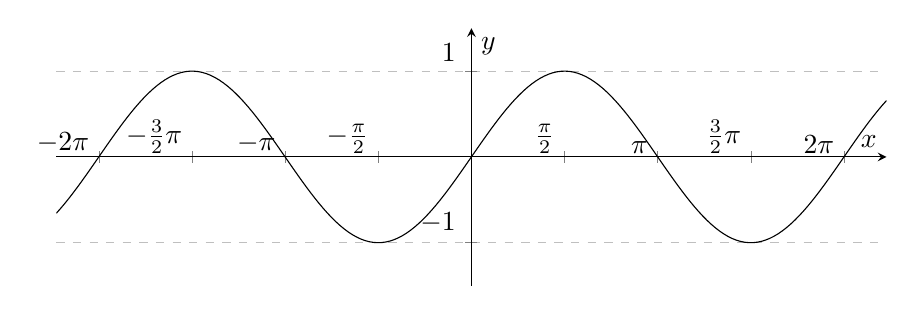
\begin{tikzpicture}
\begin{axis}[xmax = 7, xmin = -7, ymax = 1.5, ymin = -1.5,
             axis lines=middle, xlabel=$x$, ylabel=$y$,
             xtick={-2*pi, -3*pi/2, -pi, -pi/2, 0, pi/2, pi, 3*pi/2, 2*pi},
             xticklabels={$-2\pi$, $-\frac{3}{2}\pi$, $-\pi$, $-\frac{\pi}{2}$, $0$, $\frac{\pi}{2}$, $\pi$, $\frac{3}{2}\pi$, $2\pi$},
             xticklabel style={anchor=south east},
             ytick={-1, 1},
             yticklabel style={anchor=south east},
             ymajorgrids=true,
             grid style=dashed,
             width=\linewidth,
             height=0.4\linewidth
            ]
\addplot[domain=-7:7, samples=200]{sin(deg(x))};
\end{axis}
\end{tikzpicture}
\caption{Grafico di $y= \sin{x}$}
\end{figure}

\begin{figure}
\centering
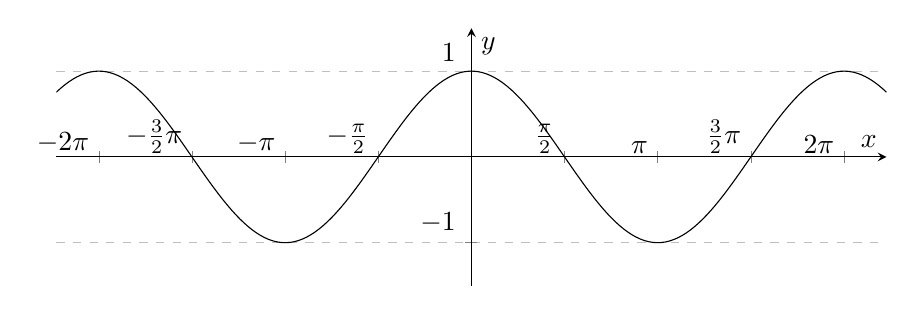
\begin{tikzpicture}
\begin{axis}[xmax = 7, xmin = -7, ymax = 1.5, ymin = -1.5,
             axis lines=middle, xlabel=$x$, ylabel=$y$,
             xtick={-2*pi, -3*pi/2, -pi, -pi/2, 0, pi/2, pi, 3*pi/2, 2*pi},
             xticklabels={$-2\pi$, $-\frac{3}{2}\pi$, $-\pi$, $-\frac{\pi}{2}$, $0$, $\frac{\pi}{2}$, $\pi$, $\frac{3}{2}\pi$, $2\pi$},
             xticklabel style={anchor=south east},
             ytick={-1, 1},
             yticklabel style={anchor=south east},
             ymajorgrids=true,
             grid style=dashed,
             width=\linewidth,
             height=0.4\linewidth
            ]
\addplot[domain=-7:7, samples=200]{cos(deg(x))};
\end{axis}
\end{tikzpicture}
\caption{Grafico di $y= \cos{x}$}
\end{figure}

\begin{figure}[H]
\centering
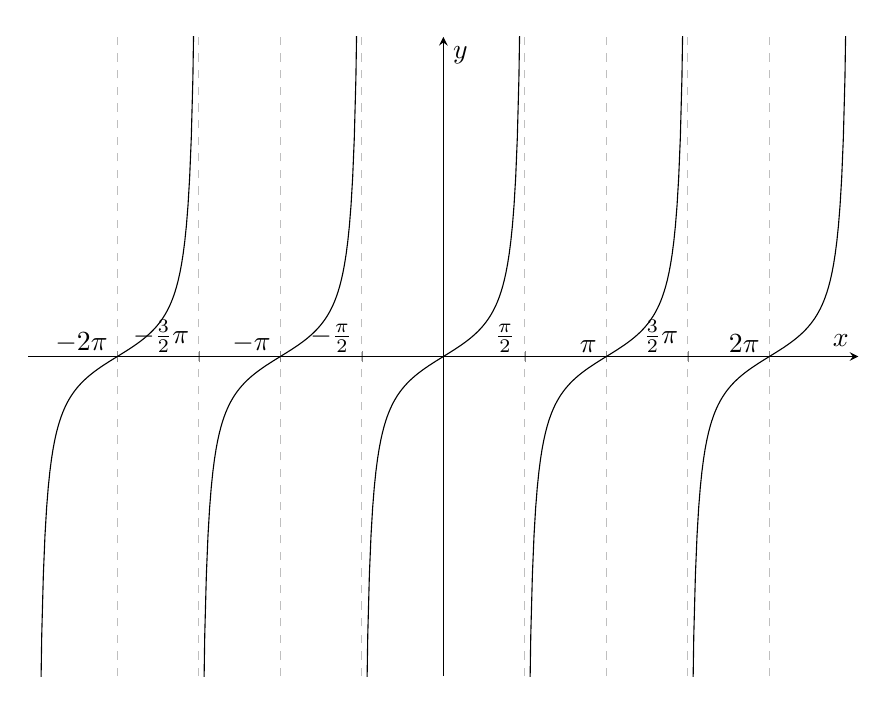
\begin{tikzpicture}
\begin{axis}[xmax = 8, xmin = -8, ymax = 10, ymin = -10,
             axis lines=middle, xlabel=$x$, ylabel=$y$,
             xtick={-2*pi, -3*pi/2, -pi, -pi/2, 0, pi/2, pi, 3*pi/2, 2*pi},
             xticklabels={$-2\pi$, $-\frac{3}{2}\pi$, $-\pi$, $-\frac{\pi}{2}$, $0$, $\frac{\pi}{2}$, $\pi$, $\frac{3}{2}\pi$, $2\pi$},
             y tick style={draw=none},
             yticklabels={},
             xticklabel style={anchor=south east},
             xmajorgrids=true,
             grid style=dashed,
             width=\linewidth,
             height=0.8\linewidth
            ]
\addplot[domain=-pi/2+0.02:pi/2-0.02, samples=100]{tan(deg(x))};
\addplot[domain=-pi/2+0.02+pi:pi/2-0.02+pi, samples=100]{tan(deg(x))};
\addplot[domain=-pi/2+0.02-pi:pi/2-0.02-pi, samples=100]{tan(deg(x))};
\addplot[domain=-pi/2+0.02+2*pi:pi/2-0.02+2*pi, samples=100]{tan(deg(x))};
\addplot[domain=-pi/2+0.02-2*pi:pi/2-0.02-2*pi, samples=100]{tan(deg(x))};
\end{axis}
\end{tikzpicture}
\caption{Grafico di $y= \tan{x}$}
\end{figure}

\subsubsection{Formule utili}
Dalla prima identità è possibile ricavare una formula per passare dal seno al coseno, il problema è che per farlo bisogna prima sapere in che quadrante ci si trova e, di conseguenza, decidere il segno della radice:
\begin{equation*}
    \sin{x} = \pm \sqrt{1-\cos^2{x}}
\end{equation*}

Di seguito le formule di \textbf{addizione} e \textbf{sottrazione}: \label{sec_formuleAddSott}
\begin{gather*}
    \cos(\alpha + \beta) = \cos{\alpha}\cos{\beta} - \sin{\alpha}\sin{\beta}\\
    \cos(\alpha - \beta) = \cos{\alpha}\cos{\beta} + \sin{\alpha}\sin{\beta}\\
    \sin(\alpha + \beta) = \sin{\alpha}\cos{\beta} + \cos{\alpha}\sin{\beta}\\
    \sin(\alpha - \beta) = \sin{\alpha}\cos{\beta} - \cos{\alpha}\sin{\beta}
\end{gather*}

Formule di \textbf{duplicazione}:\label{sec_formuleDuplicazione}
\begin{align*}
    \sin(2\alpha) &= 2\sin{\alpha}\cos{\alpha}\\
    \cos(2\alpha) &= \cos^2{\alpha} - \sin^2{\alpha} =\\
    &= 1 - 2\sin^2{\alpha} = \\
    &= 2\cos^2{\alpha} - 1
\end{align*}
Le ultime due formule per la duplicazione del coseno sono ricavate sostituendo a $\cos^2{\alpha} - \sin^2{\alpha}$ la prima identità fondamentale ($\sin^2{x} + \cos^2{x} = 1$). Si noti come la formula di duplicazione del coseno permette di passare \textbf{da un quadrato a una funzione lineare} e viceversa.

Ulteriori formule:
\begin{gather*}
    \sin\left(\frac{\pi}{2}-\alpha\right) = \cos{\alpha}\\
    \cos\left(\frac{\pi}{2}-\alpha\right) = \sin{\alpha}\\
\end{gather*}

\subsubsection{Funzioni goniometriche inverse}

Essendo seno e coseno periodiche ovviamente non sono invertibili, in quanto per essere invertibili dovrebbero essere iniettive e suriettive. In realtà seno e coseno sono suriettive, ma non iniettive. È quindi necessario restringere il loro dominio per renderle iniettive.

Per convenzione il dominio del \textbf{seno} si restringe all'intervallo $[-\frac{\pi}{2}, \frac{\pi}{2}]$. Si noti che si potrebbe scegliere un qualsiasi altro intervallo purché il seno "ristretto" sia ancora iniettivo (es. si può prendere come intervallo $[\frac{\pi}{2}, \frac{3}{2}\pi]$ ma non $[0, \pi]$).
\begin{equation*}
    \sin |_{[-\frac{\pi}{2}, \frac{\pi}{2}]}: [-\frac{\pi}{2}, \frac{\pi}{2}] \to [-1, 1]
\end{equation*}
Essendo diventata biunivoca è possibile invertirla:
\dfn{
    La funzione inversa al seno è l'\textbf{arcoseno}:
    \begin{equation*}
        \left( \sin |_{[-\frac{\pi}{2}, \frac{\pi}{2}]} \right)^{-1} (y) = \arcsin{y}
    \end{equation*}
    \begin{equation*}
        \arcsin: [-1, 1] \to [-\frac{\pi}{2}, \frac{\pi}{2}]
    \end{equation*}
}
Essendo che il codominio dell'arcoseno è $[-\frac{\pi}{2}, \frac{\pi}{2}]$:
\begin{equation*}
    \begin{cases}
        \forall x \in [-1, 1]\\
        \sin(\arcsin{x}) = x
    \end{cases}
    \qquad \qquad
    \begin{cases}
        \forall x \in [-\frac{\pi}{2}, \frac{\pi}{2}] \;\;(\mathrm{non}\; \mathbb{R})\\
        \arcsin(\sin{x}) = x
    \end{cases}
\end{equation*}
Per esempio: $\arcsin(\sin{\pi}) = \arcsin{0} = 0 \neq \pi$.\\

Lo stesso discorso vale per il \textbf{coseno} e la \textbf{tangente}. Mente però per la tangente possiamo tenere lo stesso intervallo del seno come dominio ristretto, per il coseno è necessario usare un altro intervallo in quanto $[-\frac{\pi}{2}, \frac{\pi}{2}]$ non lo renderebbe iniettivo:
\dfn{
    La funzione inversa al coseno è l'\textbf{arcocoseno}:
    \begin{equation*}
        \left( \cos |_{[0, \pi]} \right)^{-1} (y) = \arccos{y}
    \end{equation*}
    \begin{equation*}
        \arccos: [-1, 1] \to [0, \pi]
    \end{equation*}
}

\begin{equation*}
    \begin{cases}
        \forall x \in [-1, 1]\\
        \cos(\arccos{x}) = x
    \end{cases}
    \qquad \qquad
    \begin{cases}
        \forall x \in [0, \pi] \;\;(\mathrm{non}\; \mathbb{R})\\
        \arccos(\cos{x}) = x
    \end{cases}
\end{equation*}

\dfn{
    La funzione inversa alla tangente è l'\textbf{arcotangente}:
    \begin{equation*}
        \left( \tan |_{[-\frac{\pi}{2}, \frac{\pi}{2}]} \right)^{-1} (y) = \arctan{y}
    \end{equation*}
    \begin{equation*}
        \arctan: \mathbb{R} \to [-\frac{\pi}{2}, \frac{\pi}{2}]
    \end{equation*}
}

\begin{equation*}
    \begin{cases}
        \forall x \in \mathbb{R}\\
        \tan(\arctan{x}) = x
    \end{cases}
    \qquad \qquad
    \begin{cases}
        \forall x \in [-\frac{\pi}{2}, \frac{\pi}{2}] \;\;(\mathrm{non}\; \mathbb{R})\\
        \arctan(\tan{x}) = x
    \end{cases}
\end{equation*}

I grafici delle funzioni inverse sono i seguenti:
\begin{figure}[h]
\centering
\begin{tikzpicture}
\begin{axis}[xmax = 1.5, xmin = -1.5, ymax = 2, ymin = -2,
             axis lines=middle, xlabel=$x$, ylabel=$y$,
             xtick={-1, 1},
             xticklabels={$-1$, $1$},
             xticklabel style={anchor=south east},
             ytick={-pi/2, pi/2},
             yticklabels={$-\frac{\pi}{2}$, $\frac{\pi}{2}$},
             yticklabel style={anchor=south east},
             width=0.5\linewidth,
             height=0.5\linewidth
            ]
\addplot[domain=-1:1, samples=200]{asin(x)/180*pi};
\end{axis}
\end{tikzpicture}
\caption{Grafico di $y= \arcsin{x}$}
\end{figure}

\begin{figure}[h]
\centering
\begin{tikzpicture}
\begin{axis}[xmax = 1.5, xmin = -1.5, ymax = 4, ymin = -0.5,
             axis lines=middle, xlabel=$x$, ylabel=$y$,
             xtick={-1, 1},
             xticklabels={$-1$, $1$},
             xticklabel style={anchor=north},
             ytick={pi/2, pi},
             yticklabels={$\frac{\pi}{2}$, $\pi$},
             yticklabel style={anchor=south west},
             width=0.5\linewidth,
             height=0.5\linewidth
            ]
\addplot[domain=-1:1, samples=200]{acos(x)/180*pi};
\end{axis}
\end{tikzpicture}
\caption{Grafico di $y= \arccos{x}$}
\end{figure}

\begin{figure}[h]
\centering
\begin{tikzpicture}
\begin{axis}[xmax = 15, xmin = -15, ymax = 3, ymin = -3,
             axis lines=middle, xlabel=$x$, ylabel=$y$,
             xtick style={draw=none},
             xticklabels={},
             xticklabel style={anchor=north},
             ytick={-pi/2, pi/2},
             yticklabels={$-\frac{\pi}{2}$, $\frac{\pi}{2}$},
             yticklabel style={anchor=south west},
             ymajorgrids=true,
             grid style=dashed,
             width=\linewidth,
             height=0.5\linewidth
            ]
\addplot[domain=-15:15, samples=200]{atan(x)/180*pi};
\end{axis}
\end{tikzpicture}
\caption{Grafico di $y= \arctan{x}$}
\end{figure}

\subsection{Esponenziale}
Come abbiamo ricavato dalla radice aritmetica (sezione \ref{sec_radiceAritmetica}), siamo in grado di definire l'esponenziale per un qualsiasi esponente razionale positivo. Infatti qualsiasi numero razionale positivo è esprimibile nella forma $q = \frac{m}{n}$ e quindi, sempre per la radice aritmetica:
\begin{equation*}
    a^q = a^{\frac{m}{n}} = \sqrt[n]{a^m} \qquad \forall q \in \mathbb{Q}_{+}, \forall a \in \mathbb{R}_{+},\; \mathrm{con}\; n,m \in \mathbb{N}\;\, \mathrm{e}\;\, n \neq 0
\end{equation*}
\textbf{La base dell'esponenziale è necessario che sia positiva} in quanto se non lo fosse la definizione arriverebbe ad una contraddizione. Per esempio se volessi calcolare $(-2)^3 = -8$ come un esponenziale seguendo la definizione che abbiamo:
\begin{equation*}
    (-2)^3 = (-2)^{\frac{6}{2}} = \sqrt{(-2)^6} = \sqrt{64} = 8 \neq -8
\end{equation*}
Il primo passo per estendere questa definizione è chiederci come possiamo definire l'esponenziale per tutto l'insieme dei razionali, cioè anche per esponenti razionali negativi. La risposta è abbastanza semplice perché ci basta dire che se l'esponente è negativo calcoliamo il reciproco con l'esponente positivo:
\begin{equation*}
    a^{-q} = a^{-\frac{m}{n}} = \dfrac{1}{a^{\frac{m}{n}}} = \dfrac{1}{\sqrt[n]{a^m}} \qquad \forall q \in \mathbb{Q}_{+}, \forall a \in \mathbb{R}_{+},\; \mathrm{con}\; n,m \in \mathbb{N}\;\, \mathrm{e}\;\, n \neq 0
\end{equation*}
Siamo quindi riusciti a definire l'esponenziale per tutti gli esponenti razionali, sia positivi che negativi. Ora ci manca estendere questa definizione ai numeri reali. Purtroppo per farlo sono necessarie due nozioni non ancora introdotte: quella di successione e quella di limite. Per comprendere quindi a pieno i passaggi successivi è necessario andare prima guardarsi le sezioni relative (cioè la sezione \ref{sec_successioni} per le successioni e la sezione \ref{sec_limiti} per i limiti).\\

La domanda è come facciamo a definire $3^{\sqrt{2}}$ o $5^{\sqrt{27}}$? Cioè come facciamo a definire l'esponenziale per gli esponenti appartenenti all'insieme $\mathbb{R}\setminus\mathbb{Q}$? L'idea è di \textbf{approssimare l'esponente con una successione} di numeri razionali. Se per esempio voglio calcolare $3^{\sqrt{2}}$, ho come esponente $\sqrt{2}$, quindi la successione diventa:
\begin{align*}
    q_1 &= 1\\
    q_2 &= 1,4\\
    q_3 &= 1,41\\
    q_4 &= 1,414\\
    q_5 &= 1,4142\\
    q_6 &= 1,41421\\
    \vdots
\end{align*}
È facile vedere che questa successione è \textbf{crescente} ($3^{q_n} \leq 3^{q_{n+1}}$) visto che il termine successivo ha sempre una cifra in più e inoltre questa successione è \textbf{superiormente limitata} visto che $3^{q_n} \leq 3^2 = 9$. Essendo crescente e superiormente limitata questa successione ha limite e quindi $3^{\sqrt{2}}$ si definisce proprio come il limite di questa successione:
\begin{equation*}
    3^{\sqrt{2}} \vcentcolon = \lim_{n\to +\infty} 3^{q_n}
\end{equation*}
Arriviamo quindi a definire il caso generale dell'esponenziale: \label{sec_esponenziale}
\dfn{
    Si definisce \textbf{esponenziale} in base $a$ di $x$ ($\exp_a{x}$) e si indica con $a^x$, $\forall a > 0 \in \mathbb{R}$:
    \begin{enumerate}
        \item Se $x \in \mathbb{Q}_{+}$:
            \begin{equation*}
                a^x = a^{\frac{m}{n}} = \sqrt[n]{a^m} \qquad \mathrm{con}\; n,m \in \mathbb{N}: x = \frac{m}{n}\;\, \mathrm{e}\;\, n \neq 0
            \end{equation*}
        \item Se $x \in \mathbb{Q}_{-}$:
            \begin{equation*}
                a^{x} = a^{-\frac{m}{n}} = \dfrac{1}{a^{\frac{m}{n}}} = \dfrac{1}{\sqrt[n]{a^m}} \qquad \mathrm{con}\; n,m \in \mathbb{N}: x = -\frac{m}{n}\;\, \mathrm{e}\;\, n \neq 0
            \end{equation*}
        \item Se $x \in \mathbb{R}\setminus\mathbb{Q}$:\\
            Data $(q_n)_n \subseteq \mathbb{Q} : q_n \nearrow, q_n \to x$:
            \begin{equation*}
                a^x \vcentcolon = \lim_{n \to +\infty} a^{q_n}
            \end{equation*}
    \end{enumerate}
}

\imp{\begin{center}
    L'esponenziale in \textbf{base naturale} è quello in base $e$
\end{center}}
Il numero $e$ è descritto nella sezione relativa al numero di Eulero (Sezione \ref{sec_numeroDiEulero}) e si dice che l'esponenziale in questa base è "naturale" perché ha moltissime proprietà che vedremo in seguito.

\begin{figure}
\centering
\begin{subfigure}{0.49\textwidth}
\centering
	\begin{tikzpicture}
	\begin{axis}[xmax = 5, xmin = -5, ymax = 4, ymin = -0.5,
		     axis lines=middle, xlabel=$x$, ylabel=$y$,
		     xtick style={draw=none},
		     xticklabels={},
		     ytick={1},
		     yticklabels={$1$},
		     yticklabel style={anchor=north west},
		    ]
	\addplot[domain=-5:5, samples=200]{2^x};
	\end{axis}
	\end{tikzpicture}
\end{subfigure}
\begin{subfigure}{0.49\textwidth}
\centering
	\begin{tikzpicture}
	\begin{axis}[xmax = 5, xmin = -5, ymax = 4, ymin = -0.5,
		     axis lines=middle, xlabel=$x$, ylabel=$y$, xlabel style={anchor=north west},
		     xtick style={draw=none},
		     xticklabels={},
		     ytick={1},
		     yticklabels={$1$},
		     yticklabel style={anchor=south west},
		    ]
	\addplot[domain=-5:5, samples=200]{0.5^x};
	\end{axis}
	\end{tikzpicture}
\end{subfigure}
	\caption{Grafico (da sinistra a destra) di $y= a^x$ con $a > 1$ e di $y= b^x$ con $0 < b < 1$} 
\end{figure}

\subsection{Logaritmo}
Come molte funzioni anche l'esponenziale ha una sua funzione inversa, e cioè che permette di trovare l'esponente data la base e il risultato. La funzione inversa all'esponenziale è il \textbf{logaritmo}:
\thm{
    Dato $a \in \mathbb{R}: a > 0, a \neq 1$, $\forall y \in \mathbb{R}: y > 0$, $\exists \oc x \in \mathbb{R}$: $a^x = y$. Definiamo \textbf{logaritmo} in base $a$ di $y$:
    \begin{equation*}
        \log_{a}(y) \vcentcolon = x
    \end{equation*}
    
    La funzione logaritmo ha come dominio $\mathbb{R}_{+}^* = \{r \in \mathbb{R}: r > 0\}$ e come codominio $\mathbb{R}$:
    \begin{equation*}
        \log: \mathbb{R}_{+}^* \to \mathbb{R}
    \end{equation*}
}

Essendo quindi il logaritmo l'inverso dell'esponenziale:
\begin{gather*}
    a^{\log_a(y)} = y \qquad \forall y \in \mathbb{R}_{+}^{*}\\
    \log_a(a^x) = x \qquad \forall x \in \mathbb{R}
\end{gather*}
Il logaritmo naturale, cioè in base $e$ si indica come $\ln{x}$.


\begin{figure}
\centering
\begin{subfigure}{0.49\textwidth}
\centering
	\begin{tikzpicture}
	\begin{axis}[xmax = 4, xmin = -0.5, ymax = 4, ymin = -4,
		     axis lines=middle, xlabel=$x$, ylabel=$y$, ylabel style={anchor=east},
		     ytick style={draw=none},
		     yticklabels={},
		     xtick={1},
		     xticklabels={$1$},
		     xticklabel style={anchor=north west},
		    ]
	\addplot[samples=800]{ln(x)};
	\end{axis}
	\end{tikzpicture}
\end{subfigure}
\begin{subfigure}{0.49\textwidth}
\centering
	\begin{tikzpicture}
	\begin{axis}[xmax = 4, xmin = -0.5, ymax = 4, ymin = -4,
		     axis lines=middle, xlabel=$x$, ylabel=$y$, ylabel style={anchor=east},
		     ytick style={draw=none},
		     yticklabels={},
		     xtick={1},
		     xticklabels={$1$},
		     xticklabel style={anchor=north west},
		    ]
	\addplot[samples=800]{ln(x)/ln(0.5)};
	\end{axis}
	\end{tikzpicture}
\end{subfigure}
	\caption{Grafico (da sinistra a destra) di $y= \log_a(x)$ con $ a > 1$ e di $y= \log_b(x)$ con $0 < b < 1$} 
\end{figure}

Ci sarebbe da discutere sulle proprietà del logaritmo, ma mi limiterò ad elencarle di seguito:
\imp{
	\begin{align*}
		&\log_a(x \cdot y) = \log_a(x) + \log_a (y)\\[5pt]
		&\log_a \left(\dfrac{x}{y} \right) = \log_a(x) - \log_a (y)\\[5pt]
		&\log_a \left(x^y \right) = y \cdot \log_a(x)\\[5pt]
		&\log_a \left(x \right) = \dfrac{\log_b(x)}{\log_b(a)}
	\end{align*}
}
